\chapter{Work Object}%
\label{ch:workobject}
\markboth{Work Object}{}

\begin{flushright}
	{\smaller
		\textit{Citazione}\\
		-- Autore}
\end{flushright}

\section {Introduction}
In JPAD it is possible to read an .XML file as input or generate an object whose data are written in the code. Both in the first and in the second case all needed variables are initialized with data relating the choosen aircraft. The difference between these two methos is that using an .XML file, user can to define its own aircraft having clear view about the needed data useful for the analysis.\\
Contrariwise in order to perform test of program functionality, to use a default aircraft is the most simple way to generate a work object.

\section {Input data from .XML file}
\subsection{XML File Format}
XML is a file extension for an {\itshape Extensible Markup Language (XML)} file format used to create common information formats and share both the format and the data on the World Wide Web, intranets, and elsewhere using standard ASCII text.
It is defined ``Markup Language'' due to the use of tags that describes the content. XML is considered extensible because the markup symbols are unlimited and self-defining. So it is possible to use parsonal tag for each data. \\
In this way it results relatively simple to read an .XML file.\\
The key concepts of an .XML File Format are the followings:
\begin{itemize}
\item markup symbol (tag)
\item attribute
\item tree structure
\end{itemize}

As mentioned each part of the test is contained between an opening {\bfseres markup symbol} and an end markup symbol that expressed the meaning of the test.\\

\begin{figure}[H]
\centering
{
\includegraphics[height=0.39cm]{Immagini/xml1.jpg}} 
\caption{Use of markup symbol in XML language.}
\end{figure}

In addition to tag name, the markup symbols may contain also some {\bfseries attributes} that introduce more informations such as the unit of measure.\\

\begin{figure}[H]
\centering
{
\includegraphics[height=0.4cm]{Immagini/xml2.jpg}} 
\end{figure}

An .XML file ha a tree structure where there extenal knots that branch in internal knots.
%TODO add second image


\begin{figure}[H]
\centering
{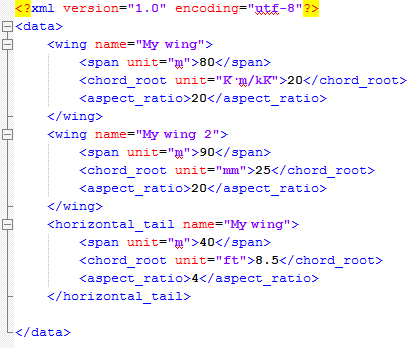
\includegraphics[height=6cm]{Immagini/xml5.jpg}} 
\caption{Tree structure of an .XML file.}
\end{figure}

\subsection{Reading data from an .XML file.}
%JPADDATAWRITER 
%possibili sviluppi futuri

\section {Default Aircraft}
\subsection {How is made a default Aircraft in JPAD}
%foto grafico 

\subsection {How is made a default Wing in JPAD}
% scrivi che è possibile costruire solo l ala come ho fatto io

\section {Database in JPAD}

In JPAD it is possible to consult external databases in .h5 format. {\bfseries HDF 5} (Hierarchical Data Format Release 5) is a data file format designed by the {\itshape National Center for Supercomputing Applications} (NCSA) to assist users in the storage and manipulation of scientific data across different operating systems and machines.\\
To obtain the useful data in JPAD  interpolating functions are used . These functions can be of one, two or three dimensions and read data from graphics that have been digitize previously.\\
Starting from these digitalizations, databases in .h5 format are built.
Reading data from databases is entrusted to methods of classes in the \texttt{database} package.\\
In order to read these databases, and obtain the useful data, it is necessary to define an object of the database reading class and associate it with the object of analysis.\\
This is a crucial step to read correctly the external data. In fact JPAD allows to work with an aircraft object  or only with an isolated lifting surface object.  Aircraft is usually composed of a fuselage, lifting surfaces, nacelle and power plant.
Furthermore, \texttt{Aircraft} and \texttt{Wing} are associated with classes of calculation like \texttt{LSAerodynamicManager} or \texttt{ACAnalysisManager}. So it is necessary that these databases are also visible from these classes.\\
So because  both in aircraft and in wing there is a lifting surface object, databases relative to wing are associated to \texttt{LSAerodynamicManager}.


\subsection {Initialize working directory tree}

First of all it is necessary to initialize the working directory tree. This step is required in order to create the following default folders that are necessary for the right behavior of the code:

\begin{itemize}
\item Database directory
\item Input directory
\item Output directory
\end{itemize}


To set the working directory with the useful folders, it's necessary to call the function \texttt{initWorkingDirectoryTree()} at the beginning of each test. The function creates all necessary folders. Morover the function has been overloaded and it can be even called with a variable number of arguments (\texttt{initWorkingDirectoryTree( String...str)}). These strings are the directory strings in \texttt{MyConfiguration} class.


\subsection {Setup database}
Here the database path it's created and associated to object that interpolates the required data from the .h5 file using a \texttt{MyInterpolatingFunction} object. After this it's possible to access the double value of the interpolating function using the \texttt{standaloneutils} method called \texttt{value}. \\


%\begin{lstlisting}[frame=rbl,caption={{\footnotesize Setup database(s)}},label= [style=\bfseries]{Listing}]
%// --------------------------------------------------------------
%// Define database
%// --------------------------------------------------------------
%MyConfiguration.initWorkingDirectoryTree();
%
%// Setup database(s)	
%String databaseFolderPath = MyConfiguration.getDir(FoldersEnum.DATABASE_DIR);
%String databaseFileName = "Aerodynamic_Database_Ultimate.h5";
%AerodynamicDatabaseReader aeroDatabaseReader = 
%		new AerodynamicDatabaseReader(
%				databaseFolderPath, 
%				databaseFileName
%				);
%\end{lstlisting}

Now the procedure to assign the database is different if is used an Aircraft object or a Wing object.

\subsection {Assign database using an Aircraft object}
In order to assign correctly the database and associate it to all analysis management is necessary to practise the following order.
\begin{enumerate}
\item Define an Aircraft Object.\\This command associates to Aircraft an object that defines the aerodynamic. From the wing it is possible to obtain the Wing, that is a \texttt{LiftingSurface} object.
\item Define an \texttt{ACAnalysisManager} object.\\All the aircraft computations are managed by this class.
\item Define an \texttt{LSAerodynamicManager} object.\\ All the lifting surfaces computations are managed by this class.
\item Associate database to \texttt{LSAerodynamicManager}.
\item Eventually do analysis.
\end{enumerate}

\subsection {Assign database using a Wing object}
Using a Wing object it isn't neccessary to define a manager for Aircraft aerodynamic analysis. So the step to follow are the same of aircraft starting from the third.
\begin{enumerate}
\item Define an Wing Object.
\item Define an \texttt{LSAerodynamicManager} object.
\item Associate database to \texttt{LSAerodynamicManager}.
\end{enumerate}

The definition of a isolated Wing is explained in the relative chapter.

%\begin{lstlisting}[frame=rbl,caption={{\footnotesize Assign database using an Aircraft object}},label= [style=\bfseries]{Listing}]
%
%// --------------------------------------------------------------
%// Generate default Aircraft
%// --------------------------------------------------------------
%Aircraft aircraft = Aircraft.createDefaultAircraft("B747-100B");
%LiftingSurface theWing = aircraft.get_wing();
%		
%// Default operating conditions
%OperatingConditions theConditions = new OperatingConditions();		
%		
%		
%// --------------------------------------------------------------
%// Define an ACAnalysisManager Object
%// --------------------------------------------------------------
%ACAnalysisManager theAnalysis = new ACAnalysisManager(theConditions);
%theAnalysis.updateGeometry(aircraft);
%		
%		
%// --------------------------------------------------------------
%// Define an LSAerodynamicsManager Object
%// --------------------------------------------------------------
%LSAerodynamicsManager theLSAnalysis = new LSAerodynamicsManager ( 
%		theConditions,
%		theWing,
%		aircraft
%		);
%		
%		
%// --------------------------------------------------------------
%// Associate database to LSAerodynamicManager
%// --------------------------------------------------------------
%theLSAnalysis.set_AerodynamicDatabaseReader(aeroDatabaseReader);
%
%		
%// --------------------------------------------------------------
%// Do analysis
%// --------------------------------------------------------------
%theAnalysis.doAnalysis(aircraft, 
%		AnalysisTypeEnum.AERODYNAMIC);
%\end{lstlisting}

\noindent \\
\begin{lstlisting}[frame=rbl,caption={{\footnotesize Assign database using an Aircraft object}},label= [style=\bfseries]{Listing}]
public static void main(String[] args) {

	// --------------------------------------------------------------
	// Define directory
	// --------------------------------------------------------------
	MyConfiguration.initWorkingDirectoryTree();


	// --------------------------------------------------------------
	// Generate default Aircraft
	// --------------------------------------------------------------
	Aircraft aircraft = Aircraft.createDefaultAircraft("B747-100B");
	LiftingSurface theWing = aircraft.get_wing();

	// Default operating conditions
	OperatingConditions theConditions = new OperatingConditions();		


	// --------------------------------------------------------------
	// Define an ACAnalysisManager Object
	// --------------------------------------------------------------
	ACAnalysisManager theAnalysis = new ACAnalysisManager(theConditions);
	theAnalysis.updateGeometry(aircraft);


	// --------------------------------------------------------------
	// Define an LSAerodynamicsManager Object
	// --------------------------------------------------------------
	LSAerodynamicsManager theLSAnalysis = new LSAerodynamicsManager ( 
			theConditions,
			theWing,
			aircraft
			);

		
	// --------------------------------------------------------------
	// Setup database(s)	
	// --------------------------------------------------------------
		
	theLSAnalysis.setDatabaseReaders(
			new Pair(DatabaseReaderEnum.AERODYNAMIC,
                          "Aerodynamic_Database_Ultimate.h5"),
			new Pair(DatabaseReaderEnum.HIGHLIFT,  
                          "HighLiftDatabase.h5")
			);

	
	// --------------------------------------------------------------
	// Do analysis
	// --------------------------------------------------------------
	theAnalysis.doAnalysis(aircraft, 
			AnalysisTypeEnum.AERODYNAMIC);
}
\end{lstlisting}
The databases are assigned to \texttt{LSAerodynamic} using a method of this class. This method accept as input a variable number of \texttt{Pair} objects.Using \texttt{Pair} objects it is possible to assign, for each database, both name and type. 

\noindent \\
\begin{lstlisting}[frame=rbl,caption={{\footnotesize \texttt{setDatabaseReaders} method}},label= [style=\bfseries]{Listing}]

public void setDatabaseReaders(Pair... args) {
	String databaseFolderPath = MyConfiguration.getDir(FoldersEnum.DATABASE_DIR);
	
	for (Pair a : args) {
		DatabaseReaderEnum key = (DatabaseReaderEnum)a.getKey(); 
		String databaseFileName = (String)a.getValue();
		
		switch (key) {
			case AERODYNAMIC:
				_aerodynamicDatabaseReader = 
				new AerodynamicDatabaseReader(
						databaseFolderPath,
						databaseFileName); 
				listDatabaseReaders.add(_aerodynamicDatabaseReader);
				break;
				
			case HIGHLIFT:
				_highLiftDatabaseReader = 
				new HighLiftDatabaseReader(
						databaseFolderPath, 
						databaseFileName); 
				listDatabaseReaders.add(_highLiftDatabaseReader);
			break;	
			
		}
\end{lstlisting}


\subsection {Developer's guide}

In order to execute some analysis in JPAD it is necessary, first of all, to define an analysis object in the Test class. The method \texttt{createDefaultAircraft} creates a new aircraft and the object that composes it. This method also populates the data of aircraft with default value corresponding to ATR-72 or Boieng 747\_100B. Moreover the method \texttt{createDefaultAircraft} calls another method in \texttt{Aircraft} class: \texttt{initialize} that initializes the objects of the classes that perform calculations. \\
The purpose of this structure is to have only a way to assign the databases at an aircraft. Inasmuch as the wing is always present, the chosen strategy is to assign the database to the aerodynamic manager of the wing.\\
In order to bring to use the database also for the aircraft calculation, it is assigned at the aerodynamic manager of the aircraft in the method called \texttt{doAnalysis}.\\
At the same time \texttt{LSAerodynamicManager} sets itself as aerodynamic in the wing object. \\
So it is possible to call the database using equally the following codes: 
\begin{itemize}
\item \texttt{theWingObject.getAerodynamics.get\_Database;}
\item \texttt{theAircraftObject.get\_theAerodynamic.get\_Database;}
\item \texttt{theLSManagerObject.get\_Database;}
\item \texttt{theACManagerObject.get\_Database;}
\end{itemize}

\begin{sidewaysfigure}

\centering
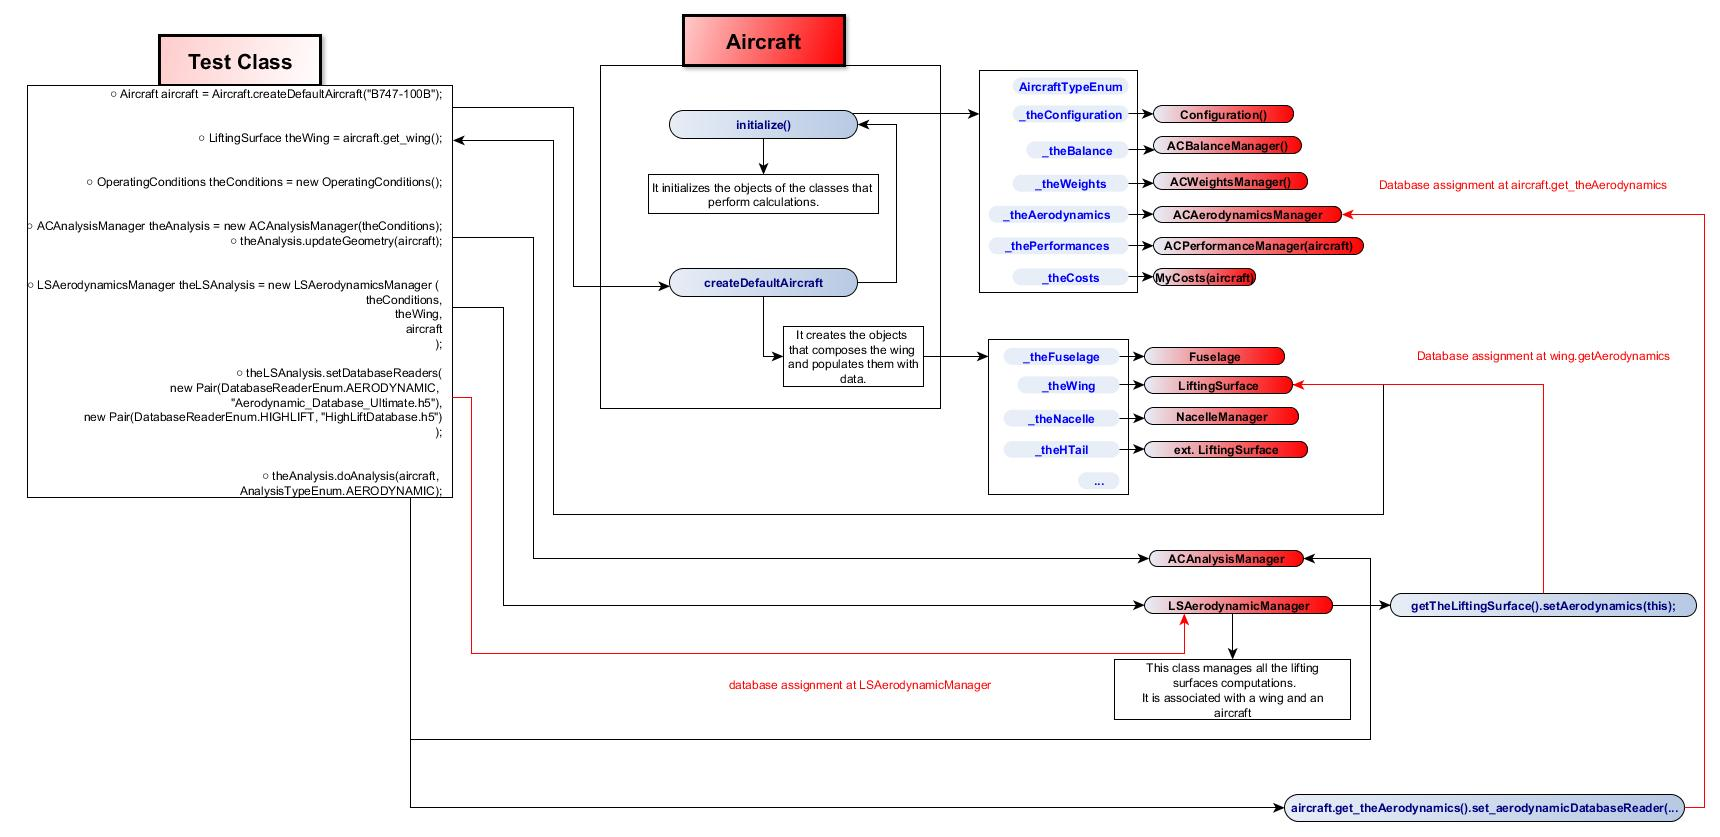
\includegraphics[width=23cm]{immagini/HowToAssignDatabase.jpg}
\caption{Flow chart of database assignment.}
\label{fig:schemauno}

\end{sidewaysfigure}